% Generated by Sphinx.
\def\sphinxdocclass{report}
\documentclass[letterpaper,10pt,english]{sphinxmanual}
\usepackage[utf8]{inputenc}
\DeclareUnicodeCharacter{00A0}{\nobreakspace}
\usepackage{cmap}
\usepackage[T1]{fontenc}
\usepackage{babel}
\usepackage{times}
\usepackage[Bjarne]{fncychap}
\usepackage{longtable}
\usepackage{sphinx}
\usepackage{multirow}


\title{Bipartite Configuration Model Documentation}
\date{January 10, 2017}
\release{1.0}
\author{Mika J. Straka}
\newcommand{\sphinxlogo}{}
\renewcommand{\releasename}{Release}
\makeindex

\makeatletter
\def\PYG@reset{\let\PYG@it=\relax \let\PYG@bf=\relax%
    \let\PYG@ul=\relax \let\PYG@tc=\relax%
    \let\PYG@bc=\relax \let\PYG@ff=\relax}
\def\PYG@tok#1{\csname PYG@tok@#1\endcsname}
\def\PYG@toks#1+{\ifx\relax#1\empty\else%
    \PYG@tok{#1}\expandafter\PYG@toks\fi}
\def\PYG@do#1{\PYG@bc{\PYG@tc{\PYG@ul{%
    \PYG@it{\PYG@bf{\PYG@ff{#1}}}}}}}
\def\PYG#1#2{\PYG@reset\PYG@toks#1+\relax+\PYG@do{#2}}

\expandafter\def\csname PYG@tok@gd\endcsname{\def\PYG@tc##1{\textcolor[rgb]{0.63,0.00,0.00}{##1}}}
\expandafter\def\csname PYG@tok@gu\endcsname{\let\PYG@bf=\textbf\def\PYG@tc##1{\textcolor[rgb]{0.50,0.00,0.50}{##1}}}
\expandafter\def\csname PYG@tok@gt\endcsname{\def\PYG@tc##1{\textcolor[rgb]{0.00,0.27,0.87}{##1}}}
\expandafter\def\csname PYG@tok@gs\endcsname{\let\PYG@bf=\textbf}
\expandafter\def\csname PYG@tok@gr\endcsname{\def\PYG@tc##1{\textcolor[rgb]{1.00,0.00,0.00}{##1}}}
\expandafter\def\csname PYG@tok@cm\endcsname{\let\PYG@it=\textit\def\PYG@tc##1{\textcolor[rgb]{0.25,0.50,0.56}{##1}}}
\expandafter\def\csname PYG@tok@vg\endcsname{\def\PYG@tc##1{\textcolor[rgb]{0.73,0.38,0.84}{##1}}}
\expandafter\def\csname PYG@tok@vi\endcsname{\def\PYG@tc##1{\textcolor[rgb]{0.73,0.38,0.84}{##1}}}
\expandafter\def\csname PYG@tok@mh\endcsname{\def\PYG@tc##1{\textcolor[rgb]{0.13,0.50,0.31}{##1}}}
\expandafter\def\csname PYG@tok@cs\endcsname{\def\PYG@tc##1{\textcolor[rgb]{0.25,0.50,0.56}{##1}}\def\PYG@bc##1{\setlength{\fboxsep}{0pt}\colorbox[rgb]{1.00,0.94,0.94}{\strut ##1}}}
\expandafter\def\csname PYG@tok@ge\endcsname{\let\PYG@it=\textit}
\expandafter\def\csname PYG@tok@vc\endcsname{\def\PYG@tc##1{\textcolor[rgb]{0.73,0.38,0.84}{##1}}}
\expandafter\def\csname PYG@tok@il\endcsname{\def\PYG@tc##1{\textcolor[rgb]{0.13,0.50,0.31}{##1}}}
\expandafter\def\csname PYG@tok@go\endcsname{\def\PYG@tc##1{\textcolor[rgb]{0.20,0.20,0.20}{##1}}}
\expandafter\def\csname PYG@tok@cp\endcsname{\def\PYG@tc##1{\textcolor[rgb]{0.00,0.44,0.13}{##1}}}
\expandafter\def\csname PYG@tok@gi\endcsname{\def\PYG@tc##1{\textcolor[rgb]{0.00,0.63,0.00}{##1}}}
\expandafter\def\csname PYG@tok@gh\endcsname{\let\PYG@bf=\textbf\def\PYG@tc##1{\textcolor[rgb]{0.00,0.00,0.50}{##1}}}
\expandafter\def\csname PYG@tok@ni\endcsname{\let\PYG@bf=\textbf\def\PYG@tc##1{\textcolor[rgb]{0.84,0.33,0.22}{##1}}}
\expandafter\def\csname PYG@tok@nl\endcsname{\let\PYG@bf=\textbf\def\PYG@tc##1{\textcolor[rgb]{0.00,0.13,0.44}{##1}}}
\expandafter\def\csname PYG@tok@nn\endcsname{\let\PYG@bf=\textbf\def\PYG@tc##1{\textcolor[rgb]{0.05,0.52,0.71}{##1}}}
\expandafter\def\csname PYG@tok@no\endcsname{\def\PYG@tc##1{\textcolor[rgb]{0.38,0.68,0.84}{##1}}}
\expandafter\def\csname PYG@tok@na\endcsname{\def\PYG@tc##1{\textcolor[rgb]{0.25,0.44,0.63}{##1}}}
\expandafter\def\csname PYG@tok@nb\endcsname{\def\PYG@tc##1{\textcolor[rgb]{0.00,0.44,0.13}{##1}}}
\expandafter\def\csname PYG@tok@nc\endcsname{\let\PYG@bf=\textbf\def\PYG@tc##1{\textcolor[rgb]{0.05,0.52,0.71}{##1}}}
\expandafter\def\csname PYG@tok@nd\endcsname{\let\PYG@bf=\textbf\def\PYG@tc##1{\textcolor[rgb]{0.33,0.33,0.33}{##1}}}
\expandafter\def\csname PYG@tok@ne\endcsname{\def\PYG@tc##1{\textcolor[rgb]{0.00,0.44,0.13}{##1}}}
\expandafter\def\csname PYG@tok@nf\endcsname{\def\PYG@tc##1{\textcolor[rgb]{0.02,0.16,0.49}{##1}}}
\expandafter\def\csname PYG@tok@si\endcsname{\let\PYG@it=\textit\def\PYG@tc##1{\textcolor[rgb]{0.44,0.63,0.82}{##1}}}
\expandafter\def\csname PYG@tok@s2\endcsname{\def\PYG@tc##1{\textcolor[rgb]{0.25,0.44,0.63}{##1}}}
\expandafter\def\csname PYG@tok@nt\endcsname{\let\PYG@bf=\textbf\def\PYG@tc##1{\textcolor[rgb]{0.02,0.16,0.45}{##1}}}
\expandafter\def\csname PYG@tok@nv\endcsname{\def\PYG@tc##1{\textcolor[rgb]{0.73,0.38,0.84}{##1}}}
\expandafter\def\csname PYG@tok@s1\endcsname{\def\PYG@tc##1{\textcolor[rgb]{0.25,0.44,0.63}{##1}}}
\expandafter\def\csname PYG@tok@ch\endcsname{\let\PYG@it=\textit\def\PYG@tc##1{\textcolor[rgb]{0.25,0.50,0.56}{##1}}}
\expandafter\def\csname PYG@tok@m\endcsname{\def\PYG@tc##1{\textcolor[rgb]{0.13,0.50,0.31}{##1}}}
\expandafter\def\csname PYG@tok@gp\endcsname{\let\PYG@bf=\textbf\def\PYG@tc##1{\textcolor[rgb]{0.78,0.36,0.04}{##1}}}
\expandafter\def\csname PYG@tok@sh\endcsname{\def\PYG@tc##1{\textcolor[rgb]{0.25,0.44,0.63}{##1}}}
\expandafter\def\csname PYG@tok@ow\endcsname{\let\PYG@bf=\textbf\def\PYG@tc##1{\textcolor[rgb]{0.00,0.44,0.13}{##1}}}
\expandafter\def\csname PYG@tok@sx\endcsname{\def\PYG@tc##1{\textcolor[rgb]{0.78,0.36,0.04}{##1}}}
\expandafter\def\csname PYG@tok@bp\endcsname{\def\PYG@tc##1{\textcolor[rgb]{0.00,0.44,0.13}{##1}}}
\expandafter\def\csname PYG@tok@c1\endcsname{\let\PYG@it=\textit\def\PYG@tc##1{\textcolor[rgb]{0.25,0.50,0.56}{##1}}}
\expandafter\def\csname PYG@tok@o\endcsname{\def\PYG@tc##1{\textcolor[rgb]{0.40,0.40,0.40}{##1}}}
\expandafter\def\csname PYG@tok@kc\endcsname{\let\PYG@bf=\textbf\def\PYG@tc##1{\textcolor[rgb]{0.00,0.44,0.13}{##1}}}
\expandafter\def\csname PYG@tok@c\endcsname{\let\PYG@it=\textit\def\PYG@tc##1{\textcolor[rgb]{0.25,0.50,0.56}{##1}}}
\expandafter\def\csname PYG@tok@mf\endcsname{\def\PYG@tc##1{\textcolor[rgb]{0.13,0.50,0.31}{##1}}}
\expandafter\def\csname PYG@tok@err\endcsname{\def\PYG@bc##1{\setlength{\fboxsep}{0pt}\fcolorbox[rgb]{1.00,0.00,0.00}{1,1,1}{\strut ##1}}}
\expandafter\def\csname PYG@tok@mb\endcsname{\def\PYG@tc##1{\textcolor[rgb]{0.13,0.50,0.31}{##1}}}
\expandafter\def\csname PYG@tok@ss\endcsname{\def\PYG@tc##1{\textcolor[rgb]{0.32,0.47,0.09}{##1}}}
\expandafter\def\csname PYG@tok@sr\endcsname{\def\PYG@tc##1{\textcolor[rgb]{0.14,0.33,0.53}{##1}}}
\expandafter\def\csname PYG@tok@mo\endcsname{\def\PYG@tc##1{\textcolor[rgb]{0.13,0.50,0.31}{##1}}}
\expandafter\def\csname PYG@tok@kd\endcsname{\let\PYG@bf=\textbf\def\PYG@tc##1{\textcolor[rgb]{0.00,0.44,0.13}{##1}}}
\expandafter\def\csname PYG@tok@mi\endcsname{\def\PYG@tc##1{\textcolor[rgb]{0.13,0.50,0.31}{##1}}}
\expandafter\def\csname PYG@tok@kn\endcsname{\let\PYG@bf=\textbf\def\PYG@tc##1{\textcolor[rgb]{0.00,0.44,0.13}{##1}}}
\expandafter\def\csname PYG@tok@cpf\endcsname{\let\PYG@it=\textit\def\PYG@tc##1{\textcolor[rgb]{0.25,0.50,0.56}{##1}}}
\expandafter\def\csname PYG@tok@kr\endcsname{\let\PYG@bf=\textbf\def\PYG@tc##1{\textcolor[rgb]{0.00,0.44,0.13}{##1}}}
\expandafter\def\csname PYG@tok@s\endcsname{\def\PYG@tc##1{\textcolor[rgb]{0.25,0.44,0.63}{##1}}}
\expandafter\def\csname PYG@tok@kp\endcsname{\def\PYG@tc##1{\textcolor[rgb]{0.00,0.44,0.13}{##1}}}
\expandafter\def\csname PYG@tok@w\endcsname{\def\PYG@tc##1{\textcolor[rgb]{0.73,0.73,0.73}{##1}}}
\expandafter\def\csname PYG@tok@kt\endcsname{\def\PYG@tc##1{\textcolor[rgb]{0.56,0.13,0.00}{##1}}}
\expandafter\def\csname PYG@tok@sc\endcsname{\def\PYG@tc##1{\textcolor[rgb]{0.25,0.44,0.63}{##1}}}
\expandafter\def\csname PYG@tok@sb\endcsname{\def\PYG@tc##1{\textcolor[rgb]{0.25,0.44,0.63}{##1}}}
\expandafter\def\csname PYG@tok@k\endcsname{\let\PYG@bf=\textbf\def\PYG@tc##1{\textcolor[rgb]{0.00,0.44,0.13}{##1}}}
\expandafter\def\csname PYG@tok@se\endcsname{\let\PYG@bf=\textbf\def\PYG@tc##1{\textcolor[rgb]{0.25,0.44,0.63}{##1}}}
\expandafter\def\csname PYG@tok@sd\endcsname{\let\PYG@it=\textit\def\PYG@tc##1{\textcolor[rgb]{0.25,0.44,0.63}{##1}}}

\def\PYGZbs{\char`\\}
\def\PYGZus{\char`\_}
\def\PYGZob{\char`\{}
\def\PYGZcb{\char`\}}
\def\PYGZca{\char`\^}
\def\PYGZam{\char`\&}
\def\PYGZlt{\char`\<}
\def\PYGZgt{\char`\>}
\def\PYGZsh{\char`\#}
\def\PYGZpc{\char`\%}
\def\PYGZdl{\char`\$}
\def\PYGZhy{\char`\-}
\def\PYGZsq{\char`\'}
\def\PYGZdq{\char`\"}
\def\PYGZti{\char`\~}
% for compatibility with earlier versions
\def\PYGZat{@}
\def\PYGZlb{[}
\def\PYGZrb{]}
\makeatother

\begin{document}

\maketitle
\tableofcontents
\phantomsection\label{index::doc}


The Bipartite Configuration Model (BiCM) is a statistical null model for binary
bipartite networks {\hyperref[index:squartini2011]{{[}Squartini2011{]}}} {\hyperref[index:saracco2015]{{[}Saracco2015{]}}}. It offers an unbiased method of analyzing node
similarities and obtaining statistically validated monopartite projections
{\hyperref[index:saracco2016]{{[}Saracco2016{]}}}.

The BiCM belongs to a series of entropy-based null model for binary biparite
networks, see also
\begin{itemize}
\item {} 
\href{https://github.com/tsakim/bipcm}{BiPCM}

\item {} 
\href{https://github.com/tsakim/birg}{BiRG}

\end{itemize}

Please consult the original articles for details about the underlying methods
and applications to user-movie and international trade databases
{\hyperref[index:saracco2016]{{[}Saracco2016{]}}}, {\hyperref[index:straka2016]{{[}Straka2016{]}}}.

An example case is illustrated in the {\hyperref[source/tutorial:tutorial]{\emph{Tutorial}}}.


\chapter{How to cite}
\label{index:bipartite-configuration-model-documentation}\label{index:how-to-cite}
If you use the \code{bicm} module, please cite its \href{https://github.com/tsakim/bicm}{location on Github} and the original articles {\hyperref[index:saracco2015]{{[}Saracco2015{]}}} and
{\hyperref[index:saracco2016]{{[}Saracco2016{]}}}.


\section{References}
\label{index:references}

\chapter{Getting Started}
\label{index:getting-started}

\section{Overview}
\label{source/overview:overview}\label{source/overview::doc}\label{source/overview:id1}
The \code{bicm} module is an implementation of the Bipartite Configuration Model
(BiCM) as described in the article {\hyperref[source/overview:saracco2016]{{[}Saracco2016{]}}}. The BiCM can be used as a
statistical null model to analyze the similarity of nodes in undirected
bipartite networks. The similarity criterion is based on the number of common
neighbors of nodes, which is expressed in terms of \(\Lambda\)-motifs in
the original article {\hyperref[source/overview:saracco2016]{{[}Saracco2016{]}}}. Subsequently, one can obtain
unbiased statistically validated monopartite projections of the original bipartite
network.

The construction of the BiCM, just like the related \href{https://github.com/tsakim/bipcm}{BiPCM} and \href{https://github.com/tsakim/birg}{BiRG} models, is based on the generation of a
grandcanonical ensemble of bipartite graphs subject to certain constraints. The
constraints can be of different types. For instance, in the case of the BiCM
the average degrees of the nodes of the input network are fixed. In the BiRG,
on the other hand, the total number of edges is constrained.

The average graph of the ensemble can be calculated analytically using the
entropy-maximization principle and provides a statistical null model, which can
be used for establishing statistically significant node similarities. In
general, they are referred to as entropy-based null models. For more
information and a detailed explanation of the underlying methods, please refer
to {\hyperref[source/overview:saracco2016]{{[}Saracco2016{]}}}.

By using the \code{bicm} module, the user can obtain the BiCM null model which
corresponds to the input matrix representing an undirected bipartite network.
To address the question of node similarity, the p-values of the observed
numbers of common neighbors can be calculated and used for statistical
verification. For an illustration and further details, please refer to
{\hyperref[source/overview:saracco2016]{{[}Saracco2016{]}}} and {\hyperref[source/overview:straka2016]{{[}Straka2016{]}}}.


\subsection{Dependencies}
\label{source/overview:dependencies}
\code{bicm} is written in \emph{Python 2.7} and uses the following modules:
\begin{itemize}
\item {} 
\href{https://github.com/tsakim/poibin}{poibin} Module for the Poisson Binomial
probability distribution

\item {} 
\href{https://www.scipy.org/}{scipy}

\item {} 
numpy

\item {} 
\href{https://docs.python.org/2/library/multiprocessing.html}{multiprocessing}

\item {} 
\href{https://docs.python.org/2/library/ctypes.html}{ctypes}

\item {} 
\href{https://docs.python.org/2/library/doctest.html}{doctest} For unit testing

\end{itemize}


\section{BiCM Quickstart}
\label{source/quickstart:bicm-quickstart}\label{source/quickstart::doc}
If you want to get started right away, go ahead and follow the summary below.  The \code{bicm} module encompasses essentially two steps for the analysis of node similarities in bipartite networks:
\begin{enumerate}
\item {} 
given an input matrix, create the biadjacency matrix of the BiCM null model

\item {} 
perform a statistical validation of the similarities of nodes in the same
layer

\end{enumerate}

The validated node similarities can be used to obtain an unbiased monopartite projection of the bipartite network, as illustrated in {\hyperref[source/quickstart:saracco2016]{{[}Saracco2016{]}}}.

For more detailed explanations of the methods, please refer to {\hyperref[source/quickstart:saracco2016]{{[}Saracco2016{]}}}, the {\hyperref[source/tutorial:tutorial]{\emph{Tutorial}}} and the {\hyperref[source/src:api]{\emph{API}}}.


\subsection{Obtaining the biadjacency matrix of the BiCM null model}
\label{source/quickstart:obtaining-the-biadjacency-matrix-of-the-bicm-null-model}
Be \code{mat} a two-dimensional binary NumPy array, which describes the
\href{https://en.wikipedia.org/w/index.php?title=Adjacency\_matrix\&oldid=751840428\#Adjacency\_matrix\_of\_a\_bipartite\_graph}{biadjacency matrix}
of an undirected bipartite network. The nodes of the two bipartite layers are
ordered along the columns and rows, respectively. In the algorithm, the two
layers are identified by the boolean values \code{True} for the \textbf{row-nodes} and
\code{False} for the \textbf{column-nodes}.

Import the module and initialize the Bipartite Configuration Model:

\begin{Verbatim}[commandchars=\\\{\}]
\PYG{g+gp}{\PYGZgt{}\PYGZgt{}\PYGZgt{} }\PYG{k+kn}{from} \PYG{n+nn}{src.bicm} \PYG{k+kn}{import} \PYG{n}{BiCM}
\PYG{g+gp}{\PYGZgt{}\PYGZgt{}\PYGZgt{} }\PYG{n}{cm} \PYG{o}{=} \PYG{n}{BiCM}\PYG{p}{(}\PYG{n}{bin\PYGZus{}mat}\PYG{o}{=}\PYG{n}{mat}\PYG{p}{)}
\end{Verbatim}

To create the biadjacency matrix of the BiCM, use:

\begin{Verbatim}[commandchars=\\\{\}]
\PYG{g+gp}{\PYGZgt{}\PYGZgt{}\PYGZgt{} }\PYG{n}{cm}\PYG{o}{.}\PYG{n}{make\PYGZus{}bicm}\PYG{p}{(}\PYG{p}{)}
\end{Verbatim}

The biadjacency matrix of the BiCM null model can be saved in \emph{\textless{}filename\textgreater{}}:

\begin{Verbatim}[commandchars=\\\{\}]
\PYG{g+gp}{\PYGZgt{}\PYGZgt{}\PYGZgt{} }\PYG{n}{cm}\PYG{o}{.}\PYG{n}{save\PYGZus{}matrix}\PYG{p}{(}\PYG{n}{cm}\PYG{o}{.}\PYG{n}{adj\PYGZus{}matrix}\PYG{p}{,} \PYG{n}{filename}\PYG{o}{=}\PYG{o}{\PYGZlt{}}\PYG{n}{filename}\PYG{o}{\PYGZgt{}}\PYG{p}{,} \PYG{n}{delim}\PYG{o}{=}\PYG{l+s+s1}{\PYGZsq{}}\PYG{l+s+se}{\PYGZbs{}t}\PYG{l+s+s1}{\PYGZsq{}}\PYG{p}{)}
\end{Verbatim}

By default, the file is saved in a human-readable CSV format. The information can also be saved as a binary NumPy file \code{.npy} by using:

\begin{Verbatim}[commandchars=\\\{\}]
\PYG{g+gp}{\PYGZgt{}\PYGZgt{}\PYGZgt{} }\PYG{n}{cm}\PYG{o}{.}\PYG{n}{save\PYGZus{}matrix}\PYG{p}{(}\PYG{n}{cm}\PYG{o}{.}\PYG{n}{adj\PYGZus{}matrix}\PYG{p}{,} \PYG{n}{filename}\PYG{o}{=}\PYG{o}{\PYGZlt{}}\PYG{n}{filename}\PYG{o}{\PYGZgt{}}\PYG{p}{,} \PYG{n}{binary}\PYG{o}{=}\PYG{n+nb+bp}{True}\PYG{p}{)}
\end{Verbatim}


\subsection{Calculating the p-values of the node similarities}
\label{source/quickstart:calculating-the-p-values-of-the-node-similarities}
In order to analyze the similarity of the row-layer nodes and to save the
p-values of the corresponding \(\Lambda\)-motifs, i.e. of the number of
shared neighbors {\hyperref[source/quickstart:saracco2016]{{[}Saracco2016{]}}}, use:

\begin{Verbatim}[commandchars=\\\{\}]
\PYG{g+gp}{\PYGZgt{}\PYGZgt{}\PYGZgt{} }\PYG{n}{cm}\PYG{o}{.}\PYG{n}{lambda\PYGZus{}motifs}\PYG{p}{(}\PYG{n+nb+bp}{True}\PYG{p}{,} \PYG{n}{filename}\PYG{o}{=}\PYG{l+s+s1}{\PYGZsq{}}\PYG{l+s+s1}{p\PYGZus{}values\PYGZus{}True.csv}\PYG{l+s+s1}{\PYGZsq{}}\PYG{p}{,} \PYG{n}{delim}\PYG{o}{=}\PYG{l+s+s1}{\PYGZsq{}}\PYG{l+s+se}{\PYGZbs{}t}\PYG{l+s+s1}{\PYGZsq{}}\PYG{p}{)}
\end{Verbatim}

For the column-layer nodes, use:

\begin{Verbatim}[commandchars=\\\{\}]
\PYG{g+gp}{\PYGZgt{}\PYGZgt{}\PYGZgt{} }\PYG{n}{cm}\PYG{o}{.}\PYG{n}{lambda\PYGZus{}motifs}\PYG{p}{(}\PYG{n+nb+bp}{False}\PYG{p}{,} \PYG{n}{filename}\PYG{o}{=}\PYG{l+s+s1}{\PYGZsq{}}\PYG{l+s+s1}{p\PYGZus{}values\PYGZus{}False.csv}\PYG{l+s+s1}{\PYGZsq{}}\PYG{p}{,} \PYG{n}{delim}\PYG{o}{=}\PYG{l+s+s1}{\PYGZsq{}}\PYG{l+s+se}{\PYGZbs{}t}\PYG{l+s+s1}{\PYGZsq{}}\PYG{p}{)}
\end{Verbatim}

Subsequently, the p-values can be used to perform a multiple hypotheses testing
and to obtain statistically validated monopartite projections {\hyperref[source/quickstart:saracco2016]{{[}Saracco2016{]}}}.
The p-values are calculated in parallel by default, see {\hyperref[source/parallel:parallel]{\emph{Parallel Computation}}} for
details.


\section{Tutorial}
\label{source/tutorial::doc}\label{source/tutorial:tutorial}\label{source/tutorial:id1}
The tutorial will take you step by step from the biadjacency matrix of a
real-data network to the calculation of the p-values. Our example bipartite
network will be the following:

{\hfill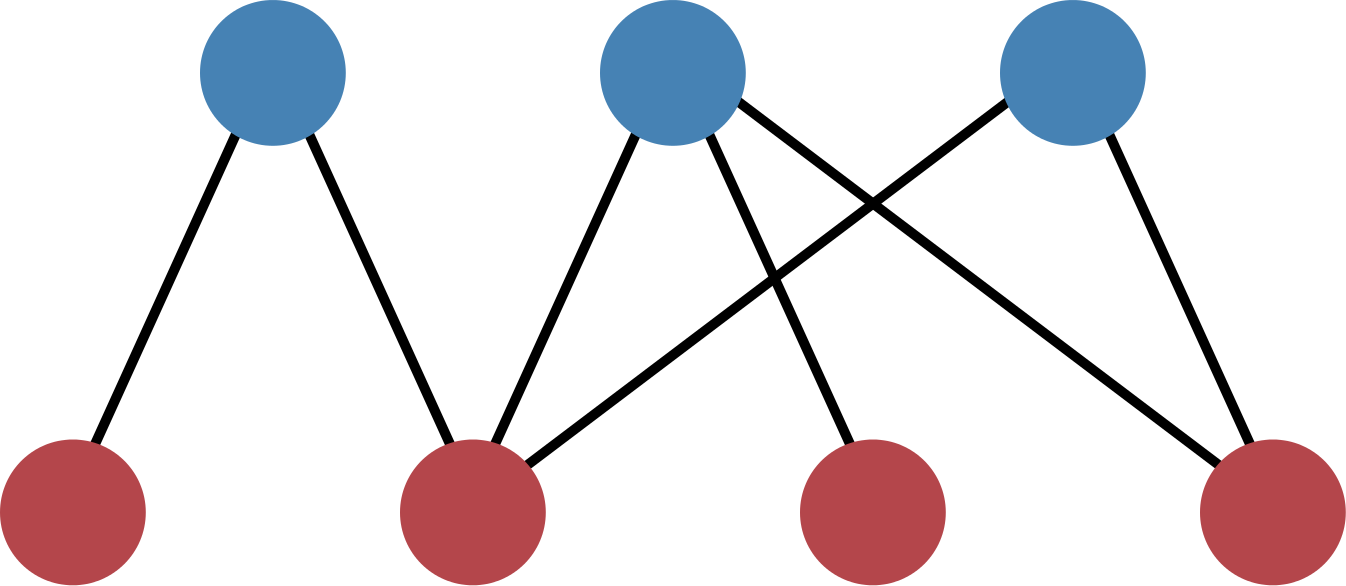
\includegraphics[width=0.250\linewidth]{nw.png}\hfill}

The structure of the network can be caught in the \href{https://en.wikipedia.org/w/index.php?title=Adjacency\_matrix\&oldid=751840428\#Adjacency\_matrix\_of\_a\_bipartite\_graph}{biadjacency matrix}.
In our case, the matrix is
\begin{gather}
\begin{split}\left[
\begin{matrix}
    1 & 1 & 0 & 0 \\
    0 & 1 & 1 & 1 \\
    0 & 1 & 0 & 1
\end{matrix}
\right]\end{split}\notag
\end{gather}
Note that the nodes of the layers of the bipartite network are ordered along
the rows and the columns, respectively. In the algorithms, the two layers are
identified by the boolean values \code{True} for the \textbf{row-nodes} and \code{False} for
the \textbf{column-nodes}. In our example image, the row-nodes are colored in blue
(top layer) and the column-nodes in red (bottom layer).

Let's get started by importing the necessary modules:

\begin{Verbatim}[commandchars=\\\{\}]
\PYG{g+gp}{\PYGZgt{}\PYGZgt{}\PYGZgt{} }\PYG{k+kn}{import} \PYG{n+nn}{numpy}
\PYG{g+gp}{\PYGZgt{}\PYGZgt{}\PYGZgt{} }\PYG{k+kn}{from} \PYG{n+nn}{src.bicm} \PYG{k+kn}{import} \PYG{n}{BiCM}
\end{Verbatim}

The biadjacency matrix of our toy network will be saved in the two-dimensional
NumPy array \code{mat}:

\begin{Verbatim}[commandchars=\\\{\}]
\PYG{g+gp}{\PYGZgt{}\PYGZgt{}\PYGZgt{} }\PYG{n}{mat} \PYG{o}{=} \PYG{n}{np}\PYG{o}{.}\PYG{n}{array}\PYG{p}{(}\PYG{p}{[}\PYG{p}{[}\PYG{l+m+mi}{1}\PYG{p}{,} \PYG{l+m+mi}{1}\PYG{p}{,} \PYG{l+m+mi}{0}\PYG{p}{,} \PYG{l+m+mi}{0}\PYG{p}{]}\PYG{p}{,}
\PYG{g+go}{                    [0, 1, 1, 1],}
\PYG{g+go}{                    [0, 1, 0, 1]])}
\end{Verbatim}

and we initialize the Bipartite Configuration Model with:

\begin{Verbatim}[commandchars=\\\{\}]
\PYG{g+gp}{\PYGZgt{}\PYGZgt{}\PYGZgt{} }\PYG{n}{cm} \PYG{o}{=} \PYG{n}{BiCM}\PYG{p}{(}\PYG{n}{bin\PYGZus{}mat}\PYG{o}{=}\PYG{n}{mat}\PYG{p}{)}
\end{Verbatim}

In order to obtain the biadjacency matrix of the BiCM null model corresponding
to the input network, a number of equations have to be solved. However, this is
done automatically by running:

\begin{Verbatim}[commandchars=\\\{\}]
\PYG{g+gp}{\PYGZgt{}\PYGZgt{}\PYGZgt{} }\PYG{n}{cm}\PYG{o}{.}\PYG{n}{make\PYGZus{}bicm}\PYG{p}{(}\PYG{p}{)}
\end{Verbatim}

You can now save the bidajacency matrix in the file \emph{\textless{}filename\textgreater{}} as:

\begin{Verbatim}[commandchars=\\\{\}]
\PYG{g+gp}{\PYGZgt{}\PYGZgt{}\PYGZgt{} }\PYG{n}{m}\PYG{o}{.}\PYG{n}{save\PYGZus{}biadjacency}\PYG{p}{(}\PYG{n}{filename}\PYG{o}{=}\PYG{o}{\PYGZlt{}}\PYG{n}{filename}\PYG{o}{\PYGZgt{}}\PYG{p}{,} \PYG{n}{delim}\PYG{o}{=}\PYG{l+s+s1}{\PYGZsq{}}\PYG{l+s+se}{\PYGZbs{}t}\PYG{l+s+s1}{\PYGZsq{}}\PYG{p}{)}
\end{Verbatim}

Note that the default delimiter is \code{\textbackslash{}t}. Other delimiters such as \code{,} or
\code{;} work fine as well. The matrix can either be saved as a human-readable
\code{.csv} or as a binary NumPy \code{.npy} file, see \code{save\_biadjacency()} in
the {\hyperref[source/src:api]{\emph{API}}}. In our example graph, the BiCM matrix should be:

\begin{Verbatim}[commandchars=\\\{\}]
\PYG{g+gp}{\PYGZgt{}\PYGZgt{}\PYGZgt{} }\PYG{n}{cm}\PYG{o}{.}\PYG{n}{adj\PYGZus{}matrix}
\PYG{g+gp}{\PYGZgt{}\PYGZgt{}\PYGZgt{} }\PYG{n}{array}\PYG{p}{(}\PYG{p}{[}\PYG{p}{[} \PYG{l+m+mf}{0.21602144}\PYG{p}{,}  \PYG{l+m+mf}{0.99855239}\PYG{p}{,}  \PYG{l+m+mf}{0.21602144}\PYG{p}{,}  \PYG{l+m+mf}{0.56873952}\PYG{p}{]}\PYG{p}{,}
\PYG{g+go}{           [ 0.56845256,  0.99969684,  0.56845256,  0.86309703],}
\PYG{g+go}{           [ 0.21602144,  0.99855239,  0.21602144,  0.56873952]])}
\end{Verbatim}

Each entry in the matrix corresponds to the probability of observing a link
between the corresponding row- and column-nodes. If we take two nodes in the
same layer, we can count the number of common neighbors that they share in the
original input network and calculate the probability of observing the same of
more common neighbors according to the BiCM {\hyperref[source/tutorial:saracco2016]{{[}Saracco2016{]}}}. This corresponds to
calculating the p-values for a right-sided hypothesis testing.

The calculation of the p-values is computation and memory intensive and should
be performed in parallel, see {\hyperref[source/parallel:parallel]{\emph{Parallel Computation}}} for details. It can be executed
by simply running:

\begin{Verbatim}[commandchars=\\\{\}]
\PYG{g+gp}{\PYGZgt{}\PYGZgt{}\PYGZgt{} }\PYG{n}{cm}\PYG{o}{.}\PYG{n}{lambda\PYGZus{}motifs}\PYG{p}{(}\PYG{o}{\PYGZlt{}}\PYG{n+nb}{bool}\PYG{o}{\PYGZgt{}}\PYG{p}{,} \PYG{n}{filename}\PYG{o}{=}\PYG{o}{\PYGZlt{}}\PYG{n}{filename}\PYG{o}{\PYGZgt{}}\PYG{p}{,} \PYG{n}{delim}\PYG{o}{=}\PYG{l+s+s1}{\PYGZsq{}}\PYG{l+s+se}{\PYGZbs{}t}\PYG{l+s+s1}{\PYGZsq{}}\PYG{p}{)}
\end{Verbatim}

where \code{\textless{}bool\textgreater{}} is either \code{True} of \code{False} depending on whether one wants
to address the similarities of the \textbf{row-} or \textbf{column-nodes}, respectively,
and \code{\textless{}filename\textgreater{}} is the name of the output file.

Having calculated the p-values, it is possible to perform a multiple hypothesis
testing with FDR control and to obtain an unbiased monopartite projection of
the original bipartite network. In the projection, only statistically
significant edges are kept.

For further information on the post-processing and the monopartite projections,
please refer to {\hyperref[source/tutorial:saracco2016]{{[}Saracco2016{]}}}.


\section{Testing}
\label{source/testing:testing}\label{source/testing::doc}\label{source/testing:id1}
The methods in the \code{bicm} module  have been implemented using \href{https://docs.python.org/2/library/doctest.html}{doctests}. To run the tests,
execute:

\begin{Verbatim}[commandchars=\\\{\}]
\PYG{g+gp}{\PYGZgt{}\PYGZgt{}\PYGZgt{} }\PYG{n}{python} \PYG{o}{\PYGZhy{}}\PYG{n}{m} \PYG{n}{doctest} \PYG{n}{bicm\PYGZus{}tests}\PYG{o}{.}\PYG{n}{txt}
\end{Verbatim}

from the folder \emph{src} in the command line. If you want to run the tests in
verbose mode, use:

\begin{Verbatim}[commandchars=\\\{\}]
\PYG{g+gp}{\PYGZgt{}\PYGZgt{}\PYGZgt{} }\PYG{n}{python} \PYG{o}{\PYGZhy{}}\PYG{n}{m} \PYG{n}{doctest} \PYG{o}{\PYGZhy{}}\PYG{n}{v} \PYG{n}{bicm\PYGZus{}tests}\PYG{o}{.}\PYG{n}{txt}
\end{Verbatim}

Note that \emph{bicm.py} and \emph{bicm\_tests.txt} have to be in the same directory to
run the test.


\section{Parallel Computation}
\label{source/parallel::doc}\label{source/parallel:parallel}\label{source/parallel:parallel-computation}
Since the calculation of the p-values is computationally demanding, the
\code{bicm} module uses the Python \href{https://docs.python.org/2/library/multiprocessing.html}{multiprocessing} package by default
for this purpose.  The number of parallel processes depends on the number of
CPUs of the work station (see variable \code{numprocs} in the method
\code{BiCM.get\_pvalues\_q()} in the {\hyperref[source/src:api]{\emph{API}}}).

If the calculation should \textbf{not} be performed in parallel, use:

\begin{Verbatim}[commandchars=\\\{\}]
\PYG{g+gp}{\PYGZgt{}\PYGZgt{}\PYGZgt{} }\PYG{n}{cm}\PYG{o}{.}\PYG{n}{lambda\PYGZus{}motifs}\PYG{p}{(}\PYG{o}{\PYGZlt{}}\PYG{n+nb}{bool}\PYG{o}{\PYGZgt{}}\PYG{p}{,} \PYG{n}{parallel}\PYG{o}{=}\PYG{n+nb+bp}{False}\PYG{p}{)}
\end{Verbatim}

instead of:

\begin{Verbatim}[commandchars=\\\{\}]
\PYG{g+gp}{\PYGZgt{}\PYGZgt{}\PYGZgt{} }\PYG{n}{cm}\PYG{o}{.}\PYG{n}{lambda\PYGZus{}motifs}\PYG{p}{(}\PYG{o}{\PYGZlt{}}\PYG{n+nb}{bool}\PYG{o}{\PYGZgt{}}\PYG{p}{)}
\end{Verbatim}


\section{API}
\label{source/src:api}\label{source/src::doc}\label{source/src:id1}
API for the methods in the \code{bicm} module.
\index{BiCM (class in src.bicm)}

\begin{fulllineitems}
\phantomsection\label{source/src:src.bicm.BiCM}\pysiglinewithargsret{\strong{class }\code{src.bicm.}\bfcode{BiCM}}{\emph{bin\_mat}}{}
Bipartite Configuration model for undirected binary bipartite networks.

This class implements the Bipartite Configuration Model (BiCM), which can
be used as a null model for the analysis of undirected and binary bipartite
networks. The class provides methods to calculate the biadjacency matrix of
the null model and to calculate node similarities in terms of p-values.
\index{add2inqueue() (src.bicm.BiCM method)}

\begin{fulllineitems}
\phantomsection\label{source/src:src.bicm.BiCM.add2inqueue}\pysiglinewithargsret{\bfcode{add2inqueue}}{\emph{nprocs}, \emph{plam\_mat}, \emph{nlam\_mat}}{}
Add elements to the in-queue to calculate the p-values.
\begin{quote}\begin{description}
\item[{Parameters}] \leavevmode\begin{itemize}
\item {} 
\textbf{nprocs} (\emph{int}) -- number of processes running in parallel

\item {} 
\textbf{plam\_mat} (\emph{numpy.array (square matrix)}) -- array containing the list of probabilities for the
single observations of \(\Lambda\)-motifs

\item {} 
\textbf{nlam\_mat} (\emph{numpy.array (square matrix)}) -- array containing the observations of
\(\Lambda\)-motifs

\end{itemize}

\end{description}\end{quote}

\end{fulllineitems}

\index{check\_input\_matrix\_is\_binary() (src.bicm.BiCM method)}

\begin{fulllineitems}
\phantomsection\label{source/src:src.bicm.BiCM.check_input_matrix_is_binary}\pysiglinewithargsret{\bfcode{check\_input\_matrix\_is\_binary}}{}{}
Check that the input matrix is binary, i.e. entries are 0 or 1.
\begin{quote}\begin{description}
\item[{Raises AssertationError}] \leavevmode
raise an error if the input matrix is not
binary

\end{description}\end{quote}

\end{fulllineitems}

\index{equations() (src.bicm.BiCM method)}

\begin{fulllineitems}
\phantomsection\label{source/src:src.bicm.BiCM.equations}\pysiglinewithargsret{\bfcode{equations}}{\emph{xx}}{}
Return the equations of the log-likelihood maximization problem.

Note that the equations for the row-nodes depend only on the
column-nodes and vice versa, see reference mentioned in the header.
\begin{quote}\begin{description}
\item[{Parameters}] \leavevmode
\textbf{xx} (\emph{numpy.array}) -- Lagrange multipliers which have to be solved

\item[{Returns}] \leavevmode
equations to be solved (of the form \(f(x) = 0\))

\item[{Return type}] \leavevmode
numpy.array

\end{description}\end{quote}

\end{fulllineitems}

\index{get\_biadjacency\_matrix() (src.bicm.BiCM method)}

\begin{fulllineitems}
\phantomsection\label{source/src:src.bicm.BiCM.get_biadjacency_matrix}\pysiglinewithargsret{\bfcode{get\_biadjacency\_matrix}}{\emph{xx}}{}
Calculate the biadjacency matrix of the null model.

The biadjacency matrix describes the BiCM null model, i.e. the optimal
average graph \(<G>^*\) with the average link probabilities
\(<G>^*_{rc} = p_{rc}\) ,
\(p_{rc} = \frac{x_r \cdot x_c}{1.0 + x_r\cdot x_c}.\)
\(x\) are the solutions of the equation system which has to be
solved for the null model.
Note that \(r\) and \(c\) are taken from opposite bipartite
node sets, thus \(r \neq c\).
\begin{quote}\begin{description}
\item[{Parameters}] \leavevmode
\textbf{xx} (\emph{numpy.array}) -- solutions of the equation system (Lagrange multipliers)

\item[{Returns}] \leavevmode
biadjacency matrix of the null model

\item[{Return type}] \leavevmode
numpy.array

\item[{Raises ValueError}] \leavevmode
raise an error if \(p_{rc} < 0\) or
\(p_{rc} > 1\) for any \(r, c\)

\end{description}\end{quote}

\end{fulllineitems}

\index{get\_lambda\_motif\_matrix() (src.bicm.BiCM static method)}

\begin{fulllineitems}
\phantomsection\label{source/src:src.bicm.BiCM.get_lambda_motif_matrix}\pysiglinewithargsret{\strong{static }\bfcode{get\_lambda\_motif\_matrix}}{\emph{mm}, \emph{bip\_set}}{}
Return the number of \(\Lambda\)-motifs as found in \code{mm}.

Given the binary input matrix \code{mm}, count the number of
\(\Lambda\)-motifs between node couples of the bipartite layer
specified by \code{bip\_set}.
\begin{quote}\begin{description}
\item[{Parameters}] \leavevmode\begin{itemize}
\item {} 
\textbf{mm} (\emph{numpy.array}) -- binary matrix

\item {} 
\textbf{bip\_set} (\emph{bool}) -- selects row-nodes (\code{True}) or column-nodes (\code{False})

\end{itemize}

\item[{Returns}] \leavevmode
square matrix of observed \(\Lambda\)-motifs

\item[{Return type}] \leavevmode
numpy.array

\end{description}\end{quote}

\end{fulllineitems}

\index{get\_plambda\_matrix() (src.bicm.BiCM static method)}

\begin{fulllineitems}
\phantomsection\label{source/src:src.bicm.BiCM.get_plambda_matrix}\pysiglinewithargsret{\strong{static }\bfcode{get\_plambda\_matrix}}{\emph{biad\_mat}, \emph{bip\_set}}{}
Return the \(\Lambda\)-motif probability tensor for \code{bip\_set}.

Given the biadjacency matrix \code{biad\_mat},
\(\mathbf{M}_{rc} = p_{rc}\), which contains the probabilities of
row-node \emph{r} and column-node \emph{c} being linked, the method returns the
tensor

\(P(\Lambda)_{ij} = (M_{i\alpha_1} \cdot M_{j\alpha_1},
M_{i\alpha_2} \cdot M_{j\alpha_2}, ...),\)

where \((i, j)\) are two nodes of the bipartite layer \code{bip\_set}
and \(\alpha_k\) runs over the nodes in the opposite layer.
\begin{quote}\begin{description}
\item[{Parameters}] \leavevmode\begin{itemize}
\item {} 
\textbf{biad\_mat} (\emph{numpy.array}) -- biadjacency matrix

\item {} 
\textbf{bip\_set} (\emph{bool}) -- selects row-nodes (\code{True}) or column-nodes (\code{False})

\end{itemize}

\end{description}\end{quote}

\end{fulllineitems}

\index{get\_pvalues\_q() (src.bicm.BiCM method)}

\begin{fulllineitems}
\phantomsection\label{source/src:src.bicm.BiCM.get_pvalues_q}\pysiglinewithargsret{\bfcode{get\_pvalues\_q}}{\emph{plam\_mat}, \emph{nlam\_mat}, \emph{parallel=True}}{}
Calculate the p-values of the observed \(\Lambda\)-motifs.

For each number of \(\Lambda\)-motifs in \code{nlam\_mat},
construct the Poisson Binomial distribution using the corresponding
probabilities in \code{plam\_mat} and calculate the p-value.

\begin{notice}{note}{Note:}
the lower-triangular part of the output matrix is null since
the matrix is symmetric by definition.
\end{notice}
\begin{quote}\begin{description}
\item[{Parameters}] \leavevmode\begin{itemize}
\item {} 
\textbf{plam\_mat} (\emph{numpy.array (square matrix)}) -- array containing the list of probabilities for the
single observations of \(\Lambda\)-motifs

\item {} 
\textbf{nlam\_mat} (\emph{numpy.array (square matrix)}) -- array containing the observations of
\(\Lambda\)-motifs

\item {} 
\textbf{parallel} (\emph{bool}) -- if \code{True}, the calculation is executed in parallel;
if \code{False}, only one process is started

\end{itemize}

\item[{Return pval\_mat}] \leavevmode
array containing the p-values corresponding to the
\(\Lambda\)-values in \code{nlam\_mat}

\item[{Return type}] \leavevmode
numpy.array

\end{description}\end{quote}

\end{fulllineitems}

\index{jacobian() (src.bicm.BiCM method)}

\begin{fulllineitems}
\phantomsection\label{source/src:src.bicm.BiCM.jacobian}\pysiglinewithargsret{\bfcode{jacobian}}{\emph{xx}}{}
Return a NumPy array with the Jacobian of the equation system.
\begin{quote}\begin{description}
\item[{Parameters}] \leavevmode
\textbf{xx} (\emph{numpy.array}) -- Lagrange multipliers which have to be solved

\item[{Returns}] \leavevmode
Jacobian

\item[{Return type}] \leavevmode
2d numpy.array

\end{description}\end{quote}

\end{fulllineitems}

\index{lambda\_motifs() (src.bicm.BiCM method)}

\begin{fulllineitems}
\phantomsection\label{source/src:src.bicm.BiCM.lambda_motifs}\pysiglinewithargsret{\bfcode{lambda\_motifs}}{\emph{bip\_set}, \emph{parallel=True}, \emph{filename=None}, \emph{delim='t'}}{}
Calculate and save the p-values of the \(\Lambda\)-motifs.

For each node couple in the bipartite layer specified by \code{bip\_set},
\(\Lambda\)-motifs and calculate the corresponding p-value.
\begin{quote}\begin{description}
\item[{Parameters}] \leavevmode\begin{itemize}
\item {} 
\textbf{bip\_set} (\emph{bool}) -- select row-nodes (\code{True}) or column-nodes (\code{False})

\item {} 
\textbf{parallel} (\emph{bool}) -- select whether the calculation of the p-values should
be run in parallel (\code{True}) or not (\code{False})

\item {} 
\textbf{filename} -- name of the file which will contain the p-values

\item {} 
\textbf{delim} -- delimiter between entries in file, default is tab

\end{itemize}

\end{description}\end{quote}

\end{fulllineitems}

\index{make\_bicm() (src.bicm.BiCM method)}

\begin{fulllineitems}
\phantomsection\label{source/src:src.bicm.BiCM.make_bicm}\pysiglinewithargsret{\bfcode{make\_bicm}}{}{}
Create the biadjacency matrix of the BiCM null model.

Solve the log-likelihood maximization problem to obtain the BiCM
null model which respects constraints on the the degree sequence of the
input matrix.
\begin{quote}\begin{description}
\item[{Raises AssertationError}] \leavevmode
raise an error if the adjacency matrix of the
null model has different dimensions than the input matrix

\end{description}\end{quote}

\end{fulllineitems}

\index{outqueue2pval\_mat() (src.bicm.BiCM method)}

\begin{fulllineitems}
\phantomsection\label{source/src:src.bicm.BiCM.outqueue2pval_mat}\pysiglinewithargsret{\bfcode{outqueue2pval\_mat}}{\emph{nprocs}}{}
Put the results from the out-queue into the p-value matrix.

\end{fulllineitems}

\index{pval\_process\_worker() (src.bicm.BiCM method)}

\begin{fulllineitems}
\phantomsection\label{source/src:src.bicm.BiCM.pval_process_worker}\pysiglinewithargsret{\bfcode{pval\_process\_worker}}{}{}
Calculate one p-value and add the result to the out-queue.

\end{fulllineitems}

\index{save\_biadjacency() (src.bicm.BiCM method)}

\begin{fulllineitems}
\phantomsection\label{source/src:src.bicm.BiCM.save_biadjacency}\pysiglinewithargsret{\bfcode{save\_biadjacency}}{\emph{filename}, \emph{delim='t'}, \emph{binary=False}}{}
Save the biadjacendy matrix of the BiCM null model.

The matrix can either be saved as a binary NumPy \code{.npy} file or as a
human-readable CSV file.

\begin{notice}{note}{Note:}
The relative path has to be provided in the filname, e.g.
\emph{../data/biadjacency\_matrix.csv}
\end{notice}
\begin{quote}\begin{description}
\item[{Parameters}] \leavevmode\begin{itemize}
\item {} 
\textbf{filename} (\emph{str}) -- name of the output file

\item {} 
\textbf{delim} (\emph{str}) -- delimiter between values in file

\item {} 
\textbf{binary} (\emph{bool}) -- if \code{True}, save as binary \code{.npy},
otherwise as CSV a file

\end{itemize}

\end{description}\end{quote}

\end{fulllineitems}

\index{save\_matrix() (src.bicm.BiCM static method)}

\begin{fulllineitems}
\phantomsection\label{source/src:src.bicm.BiCM.save_matrix}\pysiglinewithargsret{\strong{static }\bfcode{save\_matrix}}{\emph{mat}, \emph{filename}, \emph{delim='t'}, \emph{binary=False}}{}
Save the matrix \code{mat} in the file \code{filename}.

The matrix can either be saved as a binary NumPy \code{.npy} file or as a
human-readable CSV file.

\begin{notice}{note}{Note:}
The relative path has to be provided in the filname, e.g.
\emph{../data/pvalue\_matrix.csv}
\end{notice}
\begin{quote}\begin{description}
\item[{Parameters}] \leavevmode\begin{itemize}
\item {} 
\textbf{mat} (\emph{numpy.array}) -- two-dimensional matrix

\item {} 
\textbf{filename} (\emph{str}) -- name of the output file

\item {} 
\textbf{delim} (\emph{str}) -- delimiter between values in file

\item {} 
\textbf{binary} (\emph{bool}) -- if \code{True}, save as binary \code{.npy},
otherwise as CSV a file

\end{itemize}

\end{description}\end{quote}

\end{fulllineitems}

\index{set\_degree\_seq() (src.bicm.BiCM method)}

\begin{fulllineitems}
\phantomsection\label{source/src:src.bicm.BiCM.set_degree_seq}\pysiglinewithargsret{\bfcode{set\_degree\_seq}}{}{}
Return the node degree sequence of the input matrix.
\begin{quote}\begin{description}
\item[{Returns}] \leavevmode
node degree sequence {[}degrees row-nodes, degrees column-nodes{]}

\item[{Return type}] \leavevmode
numpy.array

\end{description}\end{quote}

\end{fulllineitems}

\index{solve\_equations() (src.bicm.BiCM method)}

\begin{fulllineitems}
\phantomsection\label{source/src:src.bicm.BiCM.solve_equations}\pysiglinewithargsret{\bfcode{solve\_equations}}{\emph{eq}, \emph{jac}}{}
Solve the system of equations of the maximum log-likelihood problem.

The system of equations is solved using \code{scipy}`s root function. The
solutions correspond to the Lagrange multipliers
\begin{quote}

\(x_i = \exp(-\theta_i).\)
\end{quote}
\begin{quote}\begin{description}
\item[{Parameters}] \leavevmode\begin{itemize}
\item {} 
\textbf{eq} (\emph{numpy.array}) -- system of equations (\(f(x) = 0\))

\item {} 
\textbf{jac} (\emph{numpy.ndarray}) -- Jacobian of the system

\end{itemize}

\item[{Returns}] \leavevmode
solution of the equation system

\end{description}\end{quote}

\end{fulllineitems}

\index{test\_average\_degrees() (src.bicm.BiCM method)}

\begin{fulllineitems}
\phantomsection\label{source/src:src.bicm.BiCM.test_average_degrees}\pysiglinewithargsret{\bfcode{test\_average\_degrees}}{}{}
Test the constraints on the node degrees.

Assert that the degree sequence of the solved BiCM null model graph
corresponds to the degree sequence of the input graph.

\end{fulllineitems}

\index{triumat2flat\_idx() (src.bicm.BiCM static method)}

\begin{fulllineitems}
\phantomsection\label{source/src:src.bicm.BiCM.triumat2flat_idx}\pysiglinewithargsret{\strong{static }\bfcode{triumat2flat\_idx}}{\emph{i}, \emph{j}, \emph{n}}{}
Convert an matrix index couple to a flattened array index.

Given a square matrix of dimension \(n\) and an index couple
\((i, j)\) \emph{of the upper triangular part} of the matrix, the
function returns the index which the matrix element would have in a
flattened array.

\begin{notice}{note}{Note:}\begin{itemize}
\item {} 
\(i \in [0, ..., n - 1]\)

\item {} 
\(j \in [i + 1, ..., n - 1]\)

\item {} 
returned index \(\in [0,\, n (n - 1) / 2 - 1]\)

\end{itemize}
\end{notice}
\begin{quote}\begin{description}
\item[{Parameters}] \leavevmode\begin{itemize}
\item {} 
\textbf{i} (\emph{int}) -- row index

\item {} 
\textbf{j} (\emph{int}) -- column index

\item {} 
\textbf{n} (\emph{int}) -- dimension of the square matrix

\end{itemize}

\item[{Returns}] \leavevmode
flattened array index

\item[{Return type}] \leavevmode
int

\end{description}\end{quote}

\end{fulllineitems}


\end{fulllineitems}



\section{License}
\label{source/license::doc}\label{source/license:license}\label{source/license:id1}
MIT License

Copyright (c) 2015-2016 Mika J. Straka

Permission is hereby granted, free of charge, to any person obtaining a copy
of this software and associated documentation files (the ``Software''), to deal
in the Software without restriction, including without limitation the rights
to use, copy, modify, merge, publish, distribute, sublicense, and/or sell
copies of the Software, and to permit persons to whom the Software is
furnished to do so, subject to the following conditions:

The above copyright notice and this permission notice shall be included in all
copies or substantial portions of the Software.

THE SOFTWARE IS PROVIDED ``AS IS'', WITHOUT WARRANTY OF ANY KIND, EXPRESS OR
IMPLIED, INCLUDING BUT NOT LIMITED TO THE WARRANTIES OF MERCHANTABILITY,
FITNESS FOR A PARTICULAR PURPOSE AND NONINFRINGEMENT. IN NO EVENT SHALL THE
AUTHORS OR COPYRIGHT HOLDERS BE LIABLE FOR ANY CLAIM, DAMAGES OR OTHER
LIABILITY, WHETHER IN AN ACTION OF CONTRACT, TORT OR OTHERWISE, ARISING FROM,
OUT OF OR IN CONNECTION WITH THE SOFTWARE OR THE USE OR OTHER DEALINGS IN THE
SOFTWARE.


\section{Contact}
\label{source/contact:contact}\label{source/contact::doc}
For questions or input, please write to \href{mailto:mika.straka@imtlucca.it}{mika.straka@imtlucca.it}.


\chapter{Indices and tables}
\label{index:indices-and-tables}\begin{itemize}
\item {} 
\emph{genindex}

\item {} 
\emph{modindex}

\item {} 
\emph{search}

\end{itemize}

\begin{thebibliography}{Squartini2011}
\bibitem[Saracco2015]{Saracco2015}{\phantomsection\label{index:saracco2015} 
\href{http://www.nature.com/articles/srep10595}{F. Saracco, R. Di Clemente, A. Gabrielli, T. Squartini, Randomizing bipartite networks: the case of the World Trade Web, Scientific Reports 5, 10595 (2015)}
}
\bibitem[Saracco2016]{Saracco2016}{\phantomsection\label{index:saracco2016} 
\href{https://arxiv.org/abs/1607.02481}{F. Saracco, M. J. Straka, R. Di Clemente, A. Gabrielli, G. Caldarelli, T. Squartini, Inferring monopartite projections of bipartite networks: an entropy-based approach, arXiv preprint arXiv:1607.02481}
}
\bibitem[Squartini2011]{Squartini2011}{\phantomsection\label{index:squartini2011} 
\href{http://iopscience.iop.org/article/10.1088/1367-2630/13/8/083001}{T. Squartini, D. Garlaschelli, Analytical maximum-likelihood method to detect patterns in real networks, New Journal of Physics 13, (2011)}
}
\bibitem[Straka2016]{Straka2016}{\phantomsection\label{index:straka2016} 
\href{http://www.complexnetworks.org/BookOfAbstractCNA16.pdf}{M. J. Straka, F. Saracco, G. Caldarelli, Product Similarities in International Trade from Entropy-based Null Models, Complex Networks 2016, 130-132 (11 2016), ISBN 978-2-9557050-1-8}
}
\end{thebibliography}



\renewcommand{\indexname}{Index}
\printindex
\end{document}
